\chapter{深度学习在多模态融合中的应用}
\label{cha:deeplearning}

本章主要介绍使用深度学习进行多模态信息融合的思路、具体操作和实验结果。随着深度学习的飞速发展,包括分类、识别、检测乃至决策判断等诸多任务的记录都已经被刷新。在图片的识别中深度学习更是大显身手,展示出了惊人的威力,早已超过了传统的机器学习做法。所以本文为了突破传统的 Bag of Words 信息提取与处理的局限,引入了深度学习方法。并且我们不是使用深度学习方法直接给出分类结果,而是使用深度学习的模型来提取特征层信息,然后使用SVM分类器进行分类。这样做的原因是为了便于和其他方法在多个层次上进行融合,更加具有拓展性。

此外,本文还提出了一种将深度信息转换为图片信息的深度信息自适应正规化(Depth adaptive normalization)。深度信息自适应正规化的核心思想是对于深度图片的不同组成部分(例如目标物体、背景、噪声等部分)采用不同的正规化尺度。这种方法的优势有:可以保留目标物体与次要部分(比如背景和噪声)之间的间隔,使得目标物体形状轮廓清晰可辨;同时可以保留甚至放大目标物体内部三维形状变化的信息,使得目标物体含有的信息更加具体丰满;还可以一定程度上降低噪声和背景等对于识别结果的干扰。这种方法相比于其他深度信息到图片的编码方法相比,计算量小,不需要任何额外的信息。且可以与其他编码方法结合使用,即在这种正规化的方法之上再加入其他的编码信息。

最后,因为深度学习对于数据量需求巨大,而我们使用的多模态匹配的数据集往往具有数据量不足,过拟合的现象。为了解决前述问题,我们使用了预先在当前最大的RGB图片数据集ImageNet~\inlinecite{deng2009imagenet} 中训练的模型来辅助信息提取。同时,由于已有模型的训练集只包含RGB图片,对于颜色信息我们可以直接使用原 Pretrained 模型,而对于深度信息的提取,我们尝试预先使用现有的深度图片信息对原有模型进行微调(finetune),使它更好地适应于深度信息的提取。


\section{深度学习模型描述}
\label{sec:dModel}

在实验中我们使用了八层的深度卷积神经网络 AlexNet~\inlinecite{krizhevsky2012imagenet} 在颜色信息和深度信息中分别进行深度学习训练出一个适用于RGB的模型和一个适用于深度信息的模型,然后使用相应的模型将高层特征提取出来,使用SVM分类器和~\ref{equ:sigmoid_softmax} 式做出决策并给出分类自信度。最后与其它分类模态在决策层进行融合。
引入深度学习的意义在于,Deep Learning 在许多方面可以与传统词袋信息提取方法互相补充,有助于突破传统方法的局限。同时,深度学习最终提取出的特征由于高度压缩,维度较小。最后,在数据规模足够大的时候,深度学习能够获得远高于词袋方法的分类及识别准确率。使用深度学习与传统方法互相补充,就好比使用一个新型的、更高精度的传感器与传统的传感器联合做出决策。

AlexNet 的结构如图~\ref{fig:AlexNet} 所示(图片引自~\inlinecite{krizhevsky2012imagenet})。在实验中,我们提取 AlexNet 决策层之前的两层(分别称为fc6和fc7)作为分类信息,将其提取出来并与其它特征进行融合。之所以选择这两层作为分类信息是因为以下原因:
\begin{enumerate}
\item 原模型第八层(最后一层)为决策层,会给出图片在1000个类别中的分类结果,且包含维度过少,有较大的信息损失。
\item 原模型第六层、第七层之前的信息层维数过高(例如:第五层含有 $13 \times 13 \times 128 \times 2 = 43264$ 维,数据冗余严重。而第六层第七层加起来一共只有 $2048 \times 4 = 8192$ 维)
\item 由于决策层实际上是一个SoftMax分类器,所以决策层之前的特征层的信息往往具有很好的可分性。
\end{enumerate}


\begin{figure}[H] % use float package if you want it here
  \centering
  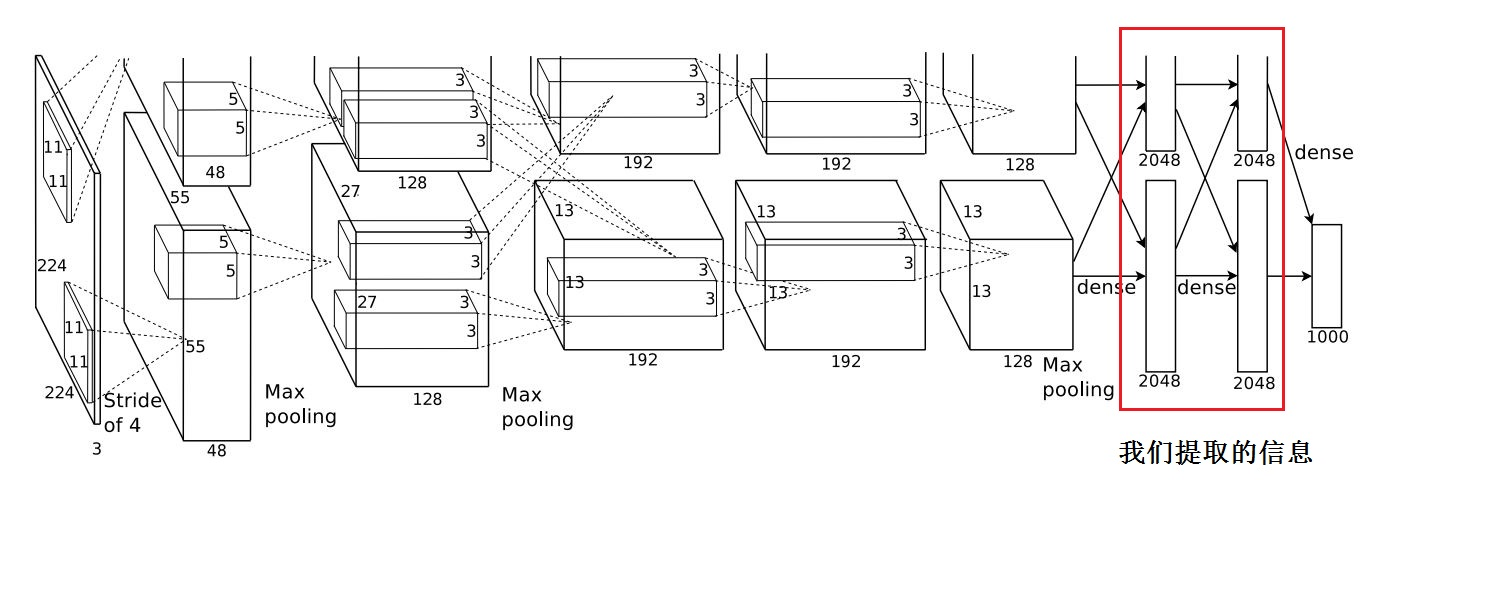
\includegraphics[width=0.95\textwidth]{AlexNet}
  \caption{AlexNet 结构示意图}
  \label{fig:AlexNet}
\end{figure}

使用上述步骤我已经可以成功地提取信息并得出分类结果。具体的参数及实验效果见~\ref{sec:deeplearningExp} 小节。


\section{Pretrained模型引入}
\label{sec:Pretrained}

在上一小节我们已经可以提取信息,不过分类效果并不是很好。这主要是因为如前所述,我们的深度学习模型因为数据量不足而发生了过拟合。所以,为了解决深度学习中数据量规模不足的问题,我们引入Pretrained模型作为辅助。我们使用的 AlexNet 模型,是 ILSVRC12 比赛中在 ImageNet 中训练出来的~\inlinecite{ILSVRC15}。

由于已有模型是在RGB图片数据集中训练的,我们在使用它处理深度信息之前一方面需要把深度信息转为合法的深度图片,另一方面会先使用已有Depth信息对其进行微调(Finetune),使它更好地适应Depth信息的提取工作。试验证明,使用RGB图片预先训练的深度学习模型可以较好地提取颜色和深度信息。使用已有模型进行微调比从头开始训练有如下好处:

\begin{enumerate}
\item 微调是在之前训练的结果的基础上继续训练,相当于数据集被扩大了,训练出的模型的表现也可以超过从头训练的模型。
\item 训练过程缩短,节省时间和资源。
\end{enumerate}

在微调过程中,我们保留 AlexNet 前七层的结构(如图~\ref{fig:AlexNet} 所示) 与参数,将第八层替换为一个输出维度为51的决策层(因为我们的数据共有51类)。以深度信息为例,从头训练与微调的训练损失(Training loss)和测试准确率(Test Accuracy)的变化对比如图~\ref{fig:training_loss} 和图~\ref{fig:accuracy} 所示,可见在微调中,原模型的训练损失迅速下降,测试准确率迅速上升,这说明原模型可以很快地适应新的数据集。

\begin{figure}[H] % use float package if you want it here
  \centering
  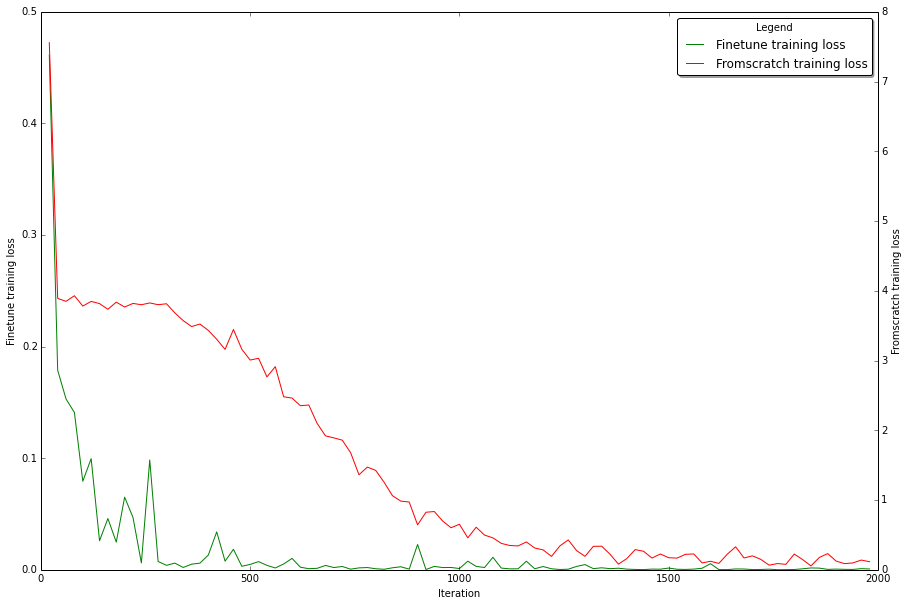
\includegraphics[width=0.95\textwidth]{training_loss}
  \caption{从头训练与微调的训练损失(Training loss)对比}
  \label{fig:training_loss}
\end{figure}

\begin{figure}[H] % use float package if you want it here
  \centering
  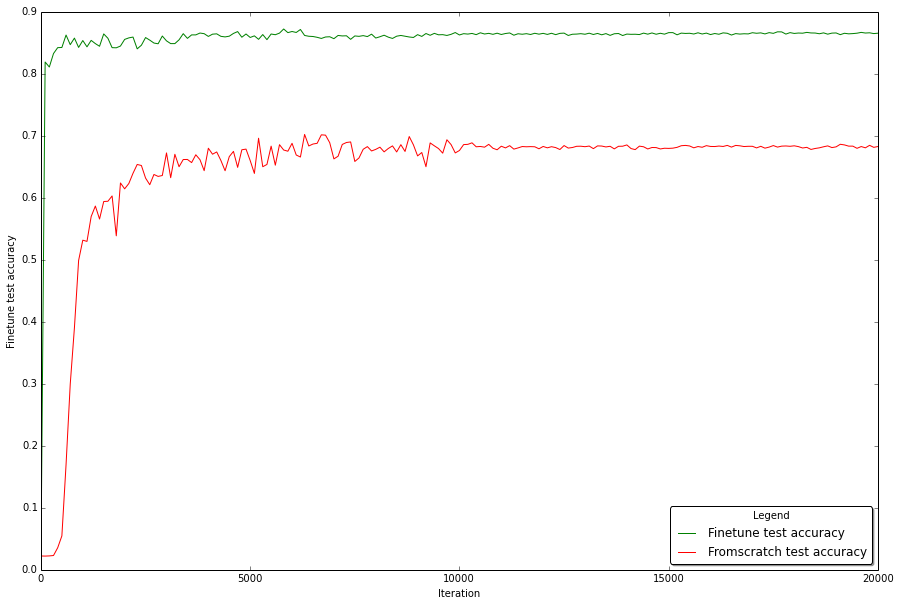
\includegraphics[width=0.95\textwidth]{accuracy}
  \caption{从头训练与微调的测试准确率(Test Accuracy)对比}
  \label{fig:accuracy}
\end{figure}

通过引入Pretrained模型,我们可以比较成功地提取RGB信息并获得85\%以上的准确率,已经接近HMP或CRNN方法中综合使用两种模态信息的表现。具体的参数及实验效果见~\ref{sec:deeplearningExp} 小节。

\section{深度信息自适应正规化}
\label{sec:dNorm}

通过引入Pretrained模型,我们已经成功地提取出RGB信息并只使用RGB信息获得85\%以上的识别准确率。然而使用深度信息效果却不甚理想,经过研究发现,这是因为我直接将深度图片传入了 Caffe 而没有将它们正规化为合法的图片。
由于深度信息是由单通道的深度数值构成的,而且每一个像素点上的数值范围可能不合法。而合法图片信息是由三通道构成的,且每一个像素点的数值在$[0-255]$之间。所以我就把深度图片正规化到了$[0-255]$之间,并将单通道扩展为三通道。不过这样做之后效果仍然不好。所以我又尝试了一些的预处理方法,比如说试图使用一些mask把背景遮住,或者使用interpolation把深度信息中的噪声点都修补上,但是效果都善乏可陈。

最后我想到,可能是正常的正规化的过程使得深度的“纹理”信息有损失。例如,原始深度图片上,物体的深度分布在$[720-780]$之间,而背景的深度分布在$[2000-3000]$之间,噪声的深度接近0。而如果把这张深度图normalize到$[0-255]$之间的话,原来分布在$[720-780]$之间的物体信息就变成了$[\frac{720}{3000} \times 255 - \frac{780}{3000} \times 255] = [61.2, 66.3]$之间,也就是说物体自身上的深度差异很大程度上被忽略了;当然,这样做也有好处,就是物体和背景之间的gap特别大,但是我觉得适当缩小gap并不会影响物体形状轮廓的可辨识度。

所以我提出了一种{\heiti 深度信息自适应正规化方法} (Depth Adaptive Normalization, DAN),会有选择地保留、加重、淡化、忽略某些信息。规范化的描述见算法~\ref{alg:DAN}。

\begin{algorithm}
  \caption{Depth Adaptive Normalization}
  \label{alg:DAN}
  \begin{algorithmic}[1]
    \REQUIRE DepthMap $\in R^{n \times m}$,\quad MaxGapNear,\quad MaxGapFar,\quad ThresholdGap
    \STATE $DepthArray \gets Squeeze(DepthMap)$
    \STATE $DepthArray \gets Sort(Unique(DepthArray))$
    \STATE targetNear $\gets$ min(DepthArray),\quad targetFar $\gets$ max(DepthArray)
    % Find the two gaps
    \\ \textbf{Find the two gaps}
    \FOR {$e_i$ in DepthArray}
      \IF {$e_i$ - $e_{i-1}$ > ThresholdGap}
        \IF {targetNear == -1}
          \STATE {targetNear $\gets e_{i}$}
        \ELSE
          \STATE {targetFar $\gets e_{i-1}$}
        \ENDIF
      \ENDIF
    \ENDFOR
    % Normalize the two gaps
    \\ \textbf{Normalize the two gaps}
    \FOR {$e_i$ in DepthMap}
      \IF {$e_i$ < targetNear}
        \STATE {$e_i \gets$ 0}
      \ELSIF {$e_i$ > targetFar}
        \STATE {$e_i \gets$ (targetFar - targetNear) + MaxGapNear + MaxGapFar}
      \ELSE
        \STATE {$e_i \gets e_i$ - (targetNear + MaxGapNear)}
      \ENDIF
    \ENDFOR
  \end{algorithmic}
\end{algorithm}

具体地说,就是先根据明显的Gap将深度信息划分为几个部分,然后根据需要保留相应的部分(比如目标物体信息),忽略不需要的部分(比如gap,背景信息),如图~\ref{fig:DAN} 所示。

\begin{figure}[H] % use float package if you want it here
  \centering
  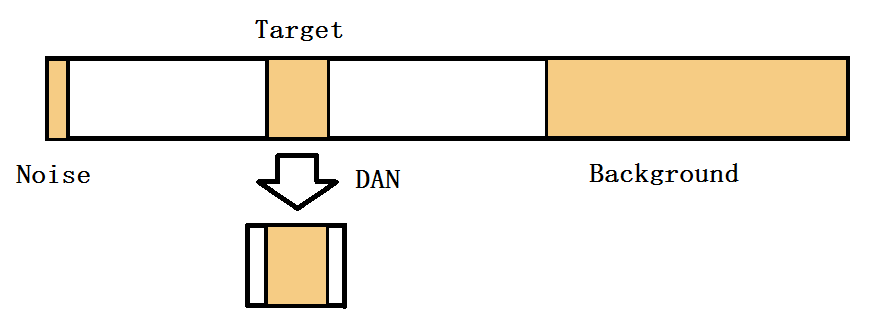
\includegraphics[width=0.95\textwidth]{DAN}
  \caption{深度信息自适应正规化方法示意图}
  \label{fig:DAN}
\end{figure}

比如说上例中,设置 $MaxGap = 20$。 0到720之间gap为720,把它缩小到20,780到2000之间gap为1280,把它缩小到20,2000到3000之间很容易判断为背景,所以这部分数值都用2000代替(不需要考虑背景的纹理)。所以最终深度信息变为$[0-20][20-80][80-100]$(其中[20-80]是原来的 $[720-780]$ 之间的物体信息),把这些信息再缩放到 $[0-255]$ 之间即完成了正规化。这样做的好处有:

\begin{enumerate}
\item 保留了目标物体与其他部分(比如背景和噪声)之间的间隔,使得目标物体形状轮廓清晰可辨。
\item 保留了(有时甚至可能放大)目标物体内部三维形状变化的信息,使得目标物体含有的信息更加具体丰满。
\item 一定程度上忽略了噪声、背景对于识别效果的干扰。
\end{enumerate}

具体的,我们将算法~\ref{alg:DAN} 中的 MaxGapNear 和 MaxGapFar 设为 5,ThresholdGap 设为100,在对水壶的深度信息处理之后可以可到的的深度图像如图~\ref{fig:DANresult} 所示,而不使用DAN得到的深度图像如图~\ref{fig:noDANresult} 所示。图~\ref{fig:DANresult} 包含了更加细致的水壶壶身弧度的变化,所以显然包含更加详细的深度信息。

\begin{figure}[htbp]
\begin{minipage}{0.48\textwidth}
  \centering
  
\includegraphics{pitchernonorm}
  \caption{使用普通正规化得到的深度图像}
  \label{fig:noDANresult}
\end{minipage}\hfill
\begin{minipage}{0.48\textwidth}
  \centering
  
\includegraphics{pitcher20}
  \caption{使用DAN得到的深度图像}
  \label{fig:DANresult}
\end{minipage}
\caption{深度信息自适应正规化效果}
\label{fig:DANcompare}
\end{figure}

通过本小节介绍的深度信息自适应正规化方法,我们可以成功提取深度信息并获得80\%以上的分类准确率。具体的参数及实验效果见~\ref{sec:deeplearningExp} 小节。

\section{试验验证}
\label{sec:deeplearningExp}

\subsection{试验综述}

华盛顿大学RGB-D数据集的物体由41877个含家用物品的RGB-D图像组织成,它们分别属于51个不同的种类和一共300个实例,这些图像是在三个不同视点捕捉的。我们使用间隔5帧的采样来评估我们的算法。我们使用和Lai等
人~\inlinecite{lai2011large} 相同的十折交叉验证分割,来评估我们的方法在类别识别任务中的表现。每个分割包括大约35000组训练RGB-D数据和7000组测试RGB-D数据。在每个分割中,每一个对象类中都有一个实例是被留下做测试的。所以我们在剩下的 300-51 = 249 个实例中进行训练。在测试时任务是给每个之前没见过的实例分类。

我们使用了开源的深度学习框架——Caffe~\inlinecite{jia2014caffe} 来完成我们深度学习的试验。
同时,我们使用Krizhevsky等人~\inlinecite{krizhevsky2012imagenet}训练的AlexNet作为预训练模型。
为了使得结果更加清晰,本章的试验采用控制变量法的方式展现。分别根据:深度学习方法(是否使用预训练的模型、是否使用深度信息自适应正规化),使用的AlexNet中的信息层(第六层、第七层、两层结合),以及微调(是否微调)为变量展示了相关实验结果。特征层融合使用的是~\ref{subsec:fInMethod} 小节中介绍的方法,决策层融合使用的是~\ref{subsec:fBetweenMethod} 小节中介绍的方法。


\subsection{试验参数}

如先前所描述,我们使用 AlexNet 作为我们融合网络的基础。它由五个卷积层(在第一、第二和第五之后需要最大池化),其次是两个完全连接层和SOFTMAX分类层。除了最后一层之外所有的层都用到了线性修正单元。
在从头训练的情境中,我们将所有信息层的参数都设置成按照一种固定学习率(learning rate)的模式在改变(最开始学习率取为0.01,经过40K次迭代后变为0.001,并在60K次迭代后停止训练)。

在微调过程中我们使用预先训练的模型的前七层(如图~\ref{fig:AlexNet} 所示)的权重和偏差来初始化我们网络的前七层,丢掉了最后的SOFTMAX分类层,将第八层替换为一个输出维度为51的决策层(因为我们的数据共有51类)。然后我们继续使用分阶段训练。在微调的情境中,我们将模型前七层的参数设置为按照一种固定学习率(learning rate)的模式在改变(最开始学习率取为0.001,经过10K次迭代后变为0.0001,并在20K次迭代后停止训练),将最后一层的学习率设置为始终是前七层的十倍(即最开始学习率取为0.01,经过10K次迭代后变为0.001,并在20K次迭代后停止训练)。这样设置的原因是前七层由于继承了原模型的参数,已经趋于稳定,需要改变的幅度较小;而第八层由于是从头训练,需要改变的幅度较大。我们尝试了微调RGB和深度信息,但是最后发现微调RGB信息并不能带来识别效果的改进。

未经特殊说明,我们将算法~\ref{alg:DAN} 中的 MaxGapNear 和 MaxGapFar 设为 5,ThresholdGap 设为100。

我们从此任务的十种数据分割方法中随机选出一种分割方法作为确认分割,而训练的迭代次数以及其他参数都是基于在确认分割上的测试结果所选定的。如果没有特殊说明,我们使用固定为0.9的momentum和固定为128的mini-batch。我们直接将图片缩放至 224 $\times$ 224 的维度,没有使用随机水平翻转。

\subsection{试验结果}

模型及方法对深度学习结果的影响如表~\ref{tab:dlResult} 所示,可以看出 Pretrained Model 可以有效提高颜色信息的分类准确率,而 Pretrained Model 加上DAN(即将深度信息正规化为合法图片)可以有效提高深度信息的分类准确率。注意,我们并没有对颜色信息使用微调。

\begin{table}[htbp]
  \centering
  \caption{模型及方法对深度学习结果的影响}
  \label{tab:dlResult}
  \begin{minipage}[t]{0.8\textwidth}
    \begin{tabularx}{\linewidth}{|l|X|X|X|}
      \hline
      \diagbox[width=9em]{方法}{模态} & RGB & Depth & RGB \& Depth \\ \hline
      From scratch      & $80.3 \pm 2.6$ & $70.7 \pm 2.3$ & $82.8 \pm 2.4$ \\
      Pretrained$^{*}$       & $\boldsymbol{85.5 \pm 1.5}$ & $76.2 \pm 2.1$ & $87.1 \pm 1.8$ \\
      Pretrained \& DAN$^{**}$  & $\boldsymbol{85.5 \pm 1.5}$ & $\boldsymbol{81.6 \pm 2.8}$ & $\boldsymbol{90.3 \pm 1.8}$ \\ \hline
    \end{tabularx}\\[2pt]
    \footnotesize
    本表展示的深度信息数据均是经过微调得到的结果,颜色和深度信息数据均是采用 fc6 \& fc7 两层信息得到的结果。\\
    *:如~\ref{sec:Pretrained} 节所述\\
    **:如~\ref{sec:dNorm} 节所述,只对深度信息使用DAN
  \end{minipage}
\end{table}

信息层对于深度学习结果的影响如表~\ref{tab:dllayerResult} 所示,可以看出使用原神经网络的第六层和第七层结合可以获得比较高的准确率和稳定性,不过这些结果与 fc6 的分类结果相比相差无几。同时我们需要考虑,fc6对于单模态信息只有4096维特征,如果加上fc7就将特征维数变为原来的两倍,而识别准确率几乎没有变化,说明fc7与fc6的信息互补性非常弱,所以在最终的综合模型中我们选择只使用fc6层信息。注意,使用其它信息层(比如fc8)并不会提高分类准确率。

\begin{table}[htbp]
  \centering
  \caption{信息层对于深度学习结果的影响}
  \label{tab:dllayerResult}
  \begin{minipage}[t]{0.8\textwidth}
    \begin{tabularx}{\linewidth}{|l|X|X|X|}
      \hline
      \diagbox[width=9em]{信息层}{模态} & RGB & Depth & RGB \& Depth \\ \hline
      fc6$^{*}$      & $85.3 \pm 1.8$ & $81.5 \pm 2.8$ & $90.2 \pm 1.7$ \\
      fc7$^{**}$     & $83.0 \pm 1.9$ & $78.8 \pm 2.6$ & $88.3 \pm 2.1$ \\
      fc6 \& fc7     & $\boldsymbol{85.5 \pm 1.5}$ & $\boldsymbol{81.6 \pm 2.8}$ & $\boldsymbol{90.3 \pm 1.8}$ \\ \hline
    \end{tabularx}\\[2pt]
    \footnotesize
    本表展示的深度信息数据均是经过DAN得到的结果,颜色和深度信息数据均是采用 Pretrained Model 得到的结果。\\
    *:fc6 是图~\ref{fig:AlexNet} 中的第六层\\
    **:fc7 是图~\ref{fig:AlexNet} 中的第七层
  \end{minipage}
\end{table}

微调对深度学习结果的影响如表~\ref{tab:dlfinetuneResult} 所示,可以看出使用深度信息微调原模型有利于深度信息的提取和利用。注意在我们的试验中微调并不会提高颜色信息的分类准确率。

\begin{table}[htbp]
  \centering
  \caption{微调对深度学习结果的影响}
  \label{tab:dlfinetuneResult}
  \begin{minipage}[t]{0.8\textwidth}
    \begin{tabularx}{\linewidth}{|l|X|X|}
      \hline
      \diagbox[width=9em]{}{模态} & Depth & RGB \& Depth \\ \hline
      不微调         & $78.1 \pm 2.1$ & $89.6 \pm 1.7$ \\
      微调           & $\boldsymbol{81.6 \pm 2.8}$ & $\boldsymbol{90.3 \pm 1.8}$ \\ \hline
    \end{tabularx}\\[2pt]
    \footnotesize
    本表展示的深度信息数据均是经过DAN得到的结果。\\
  \end{minipage}
\end{table}
